\documentclass{sig-alternate}
\newtheorem{theorem}{Theorem}[section]
\newtheorem{lemma}{Lemma}[section]
\newtheorem{definition}{Definition}[section]
\newtheorem{corollary}{Corollary}[section]
\newtheorem{proposition}{Proposition}[section]
\newtheorem{problem}{Problem}
\usepackage{algorithm}
\usepackage{algorithmic}
\usepackage{graphicx}
\usepackage{multirow}
\usepackage{subfigure}
\usepackage{verbatim} 
% \usepackage[small,compact]{titlesec}
\pdfpagewidth=8.5in
\pdfpageheight=11in
%\usepackage[small,it]{caption}
\newcommand{\squishlist}{
 \begin{list}{$\bullet$}
  { \setlength{\itemsep}{0pt}
     \setlength{\parsep}{3pt}
     \setlength{\topsep}{3pt}
     \setlength{\partopsep}{0pt}
     \setlength{\leftmargin}{1.5em}
     \setlength{\labelwidth}{1em}
     \setlength{\labelsep}{0.5em} } }

\newcommand{\squishlisttwo}{
 \begin{list}{$\bullet$}
  { \setlength{\itemsep}{0pt}
     \setlength{\parsep}{0pt}
    \setlength{\topsep}{0pt}
    \setlength{\partopsep}{0pt}
    \setlength{\leftmargin}{2em}
    \setlength{\labelwidth}{1.5em}
    \setlength{\labelsep}{0.5em} } }

\newcommand{\squishend}{
  \end{list}  }

%\setlength{\abovecaptionskip}{0pt}
%\setlength{\belowcaptionskip}{0pt} 

\begin{document}

\title{A Digital Library for Crowds on the Real-Time Social Web}

\numberofauthors{2} 
\author{
\alignauthor Jeff A. McGee\\
       \affaddr{Texas A\&M University}\\
       \affaddr{College Station, TX 77843}\\
       \email{jeffamcgee@gmail.com}
\alignauthor Krishna Y. Kamath\\
      \affaddr{Texas A\&M University}\\
       \affaddr{College Station, TX 77843}\\
       \email{kykamath@cs.tamu.edu}
}

\maketitle

\begin{abstract}
In this project, we want to build a digital library for transient crowds in highly-dynamic social messaging systems like Twitter and Facebook. A crowd is a short-lived ad-hoc collection of users, representing a ``hot-spot'' on the real-time web.  For example, an event like super-bowl might result in formation of crowds that are discussing various happenings in the game. Successful detection of these hot-spots can positively impact related research directions in online event detection, content personalization, social information discovery, etc. We will build a framework that allows an analyst or curious user to find interesting crowds and see how they evolve.  This framework will have three main parts: a database to store crowds, users, and their messages; a set of crowd detection algorithms and filters; and a tool for searching for crowds by topic, geography, or user-name.
\end{abstract}

\section{Introduction}

% \section{Related Work}
% \label{sec:reclated_work}



\section{Crowd Discovery Algorithm}
\label{sec:crowd_algorithm}
\begin{figure}
\centering
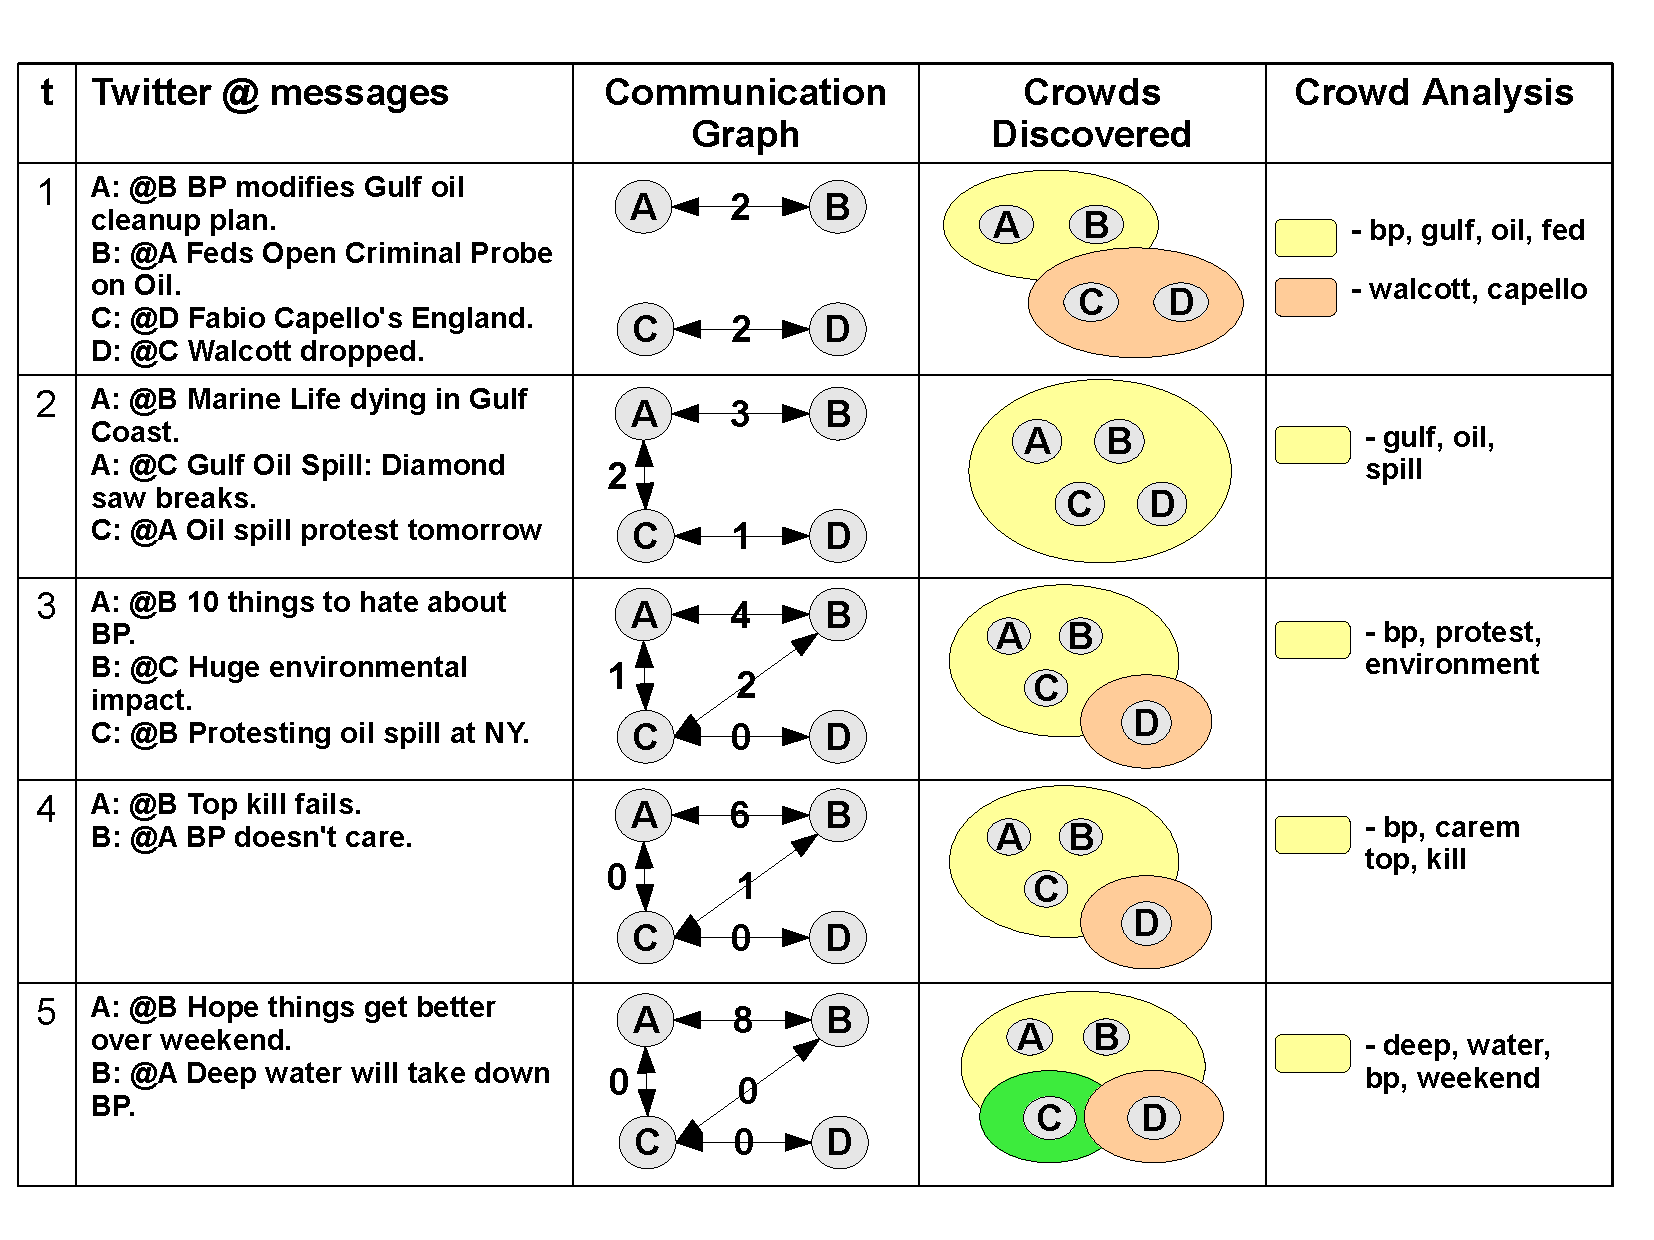
\includegraphics[width=\linewidth]{images/intro}
\caption{Example of crowd discovery and tracking in Twitter.}
\label{fig:intro-example}
\end{figure}
To illustrate the problem of crowd discovery, consider the simple example in
Figure~\ref{fig:intro-example}. At time t=1, users A and B send messages to each
other, as do users C and D.\footnote{For simplicity, the example discretizes
time so that all messages between users occur in steps. In practice, the proposed
algorithm relaxes this assumption and can handle arbitrary message sending
times.} The associated communication graph shows an edge between the two pairs,
where for simplicity the edge is annotated with the number of messages between
the users (2, in both cases). Further, suppose we identify crowds based purely on
graph connectivity. So for time t=1, we see there are two crowds discovered
\{A,B\} and \{C,D\}. For each crowd, we can characterize the semantics of their
communication with simple keywords extracted from the content of the tweets:
(``oil'', ``gulf'') and (``walcott'', ``capello''). At time t=2, the
communication graph is updated with a new edge (connecting User A and User C),
and the existing edges are decayed by one (again, a simplifying assumption for
the purposes of this example). A single crowd is discovered since all users are
connected via edges with non-zero edge weights. At time t=3, User D leaves the
main crowd since no messages to or from User D have been observed since time t=1.
This process continues until time t=5 when User C also leaves the main crowd due
to inactivity. Note that crowds are discovered from communication graph only and
not from the content of the messages. As an example of crowd tracking, we can
track the evolution of the yellow crowd across time periods, observing the
changes it goes through as it grows in size from t=1 to t=2 and then reduces to
two users by t=5.

The grouper deals with the transient crowd discovery and tracking in systems like Facebook and Twitter. For practical crowd discovery and tracking in a large time-evolving communication network, however, we face four key challenges:

\begin{list}{\labelitemi}{\leftmargin= 0.3cm}

\item First, systems like Facebook and Twitter are extremely large (on the order
of 100s of millions of unique users), placing huge demands on the computational
cost of traditional community detection approaches (which can be $O(n^3)$ in the
number of users \cite{flake:cut-clustering}).

\item Second, these services support a high-rate of edge addition (new
messages) so the discovered crowds may become stale quickly, resulting in the need to
re-identify all crowds at regular intervals (again, incurring the high cost of
community detection). The bursty nature of user communication demands a crowd
discovery approach that can capture these highly-temporal based clusters.

\item Third, the strength of association between two users may depend on many
factors (e.g., recency of communication), meaning that a crowd discovery approach
based on graph clustering should carefully consider edge weights. With no decay
at all (meaning that edges are only inserted into the network but never removed),
all users will tend towards a single trivial large crowd. Conversely, overly
aggressive edge decay may inhibit any crowd formation at all (since edges between
users may be removed nearly as soon as they are added).

\item Fourth, crowds may evolve at different rates, with some evolving over
several minutes, while others taking several days. Since crowds are inherently
ad-hoc (without unique community identifiers -- e.g., Fans of LA Lakers), the
formation, growth and dispersal of crowds must be carefully managed for
meaningful crowd analysis.
\end{list}

With these challenges in mind, we propose to discover and track transient crowds
through a communication based clustering approach over time-evolving
graphs that captures the natural conversational nature of social messaging
systems. Two of the salient features of the proposed approach are (i) an
efficient locality-based clustering approach for identifying crowds of users in
near real-time compared to more heavyweight static clustering algorithms; and
(ii) a novel crowd tracking and evolution approach for linking crowds across time
periods.

To support transient crowd discovery in Twitter-like services with 100s of
millions of participants, we propose to leverage the inherent locality in social
messaging systems. Concretely, we identify two types of locality that are
evident in Twitter-like messaging systems: (i) temporal locality and (ii) spatial
locality.

\medskip \noindent\textbf{Temporal Locality:} Transient crowds are
intuitively short-lived, since they correspond to actively communicating groups
of users. Hence, the composition of a crowd at a point-in-time should be impacted
by recent messages as opposed to older messages. As more users interact with the
crowd, the crowd should grow reflecting this \textit{temporal locality} and then
shrink as users in the crowd become inactive (that is, their last communication
with the crowd becomes more distant in time).

\medskip \noindent \textbf{Spatial Locality:} Intuitively, transient crowds are
made up of a very small percentage of users compared to the entire population of
the social network. Hence, new messages (corresponding to the addition of edges
to the communication network) should have only a local influence on the crowds
that exist at any given time. That is, changes in a small region of a graph
should not affect the entire graph. In a dataset of 61 million Twitter messages
described in \cite{Kamath:2011:TCD}, we have confirmed the existence of
this \textit{spatial locality} by finding that only about 1\% of users are within
two hops, meaning that an edge insertion has only a local effect.

\medskip Hence, we can take advantage of both, local changes to the overall
communication network (spatial locality) and recent changes to the network
(temporal locality), for supporting efficient transient crowd discovery. The complete algorithm is decsribed in \cite{Kamath:2011:TCD}


\section{Architecture}
\label{sec:architecture}
\begin{figure}[!t]
\begin{center}
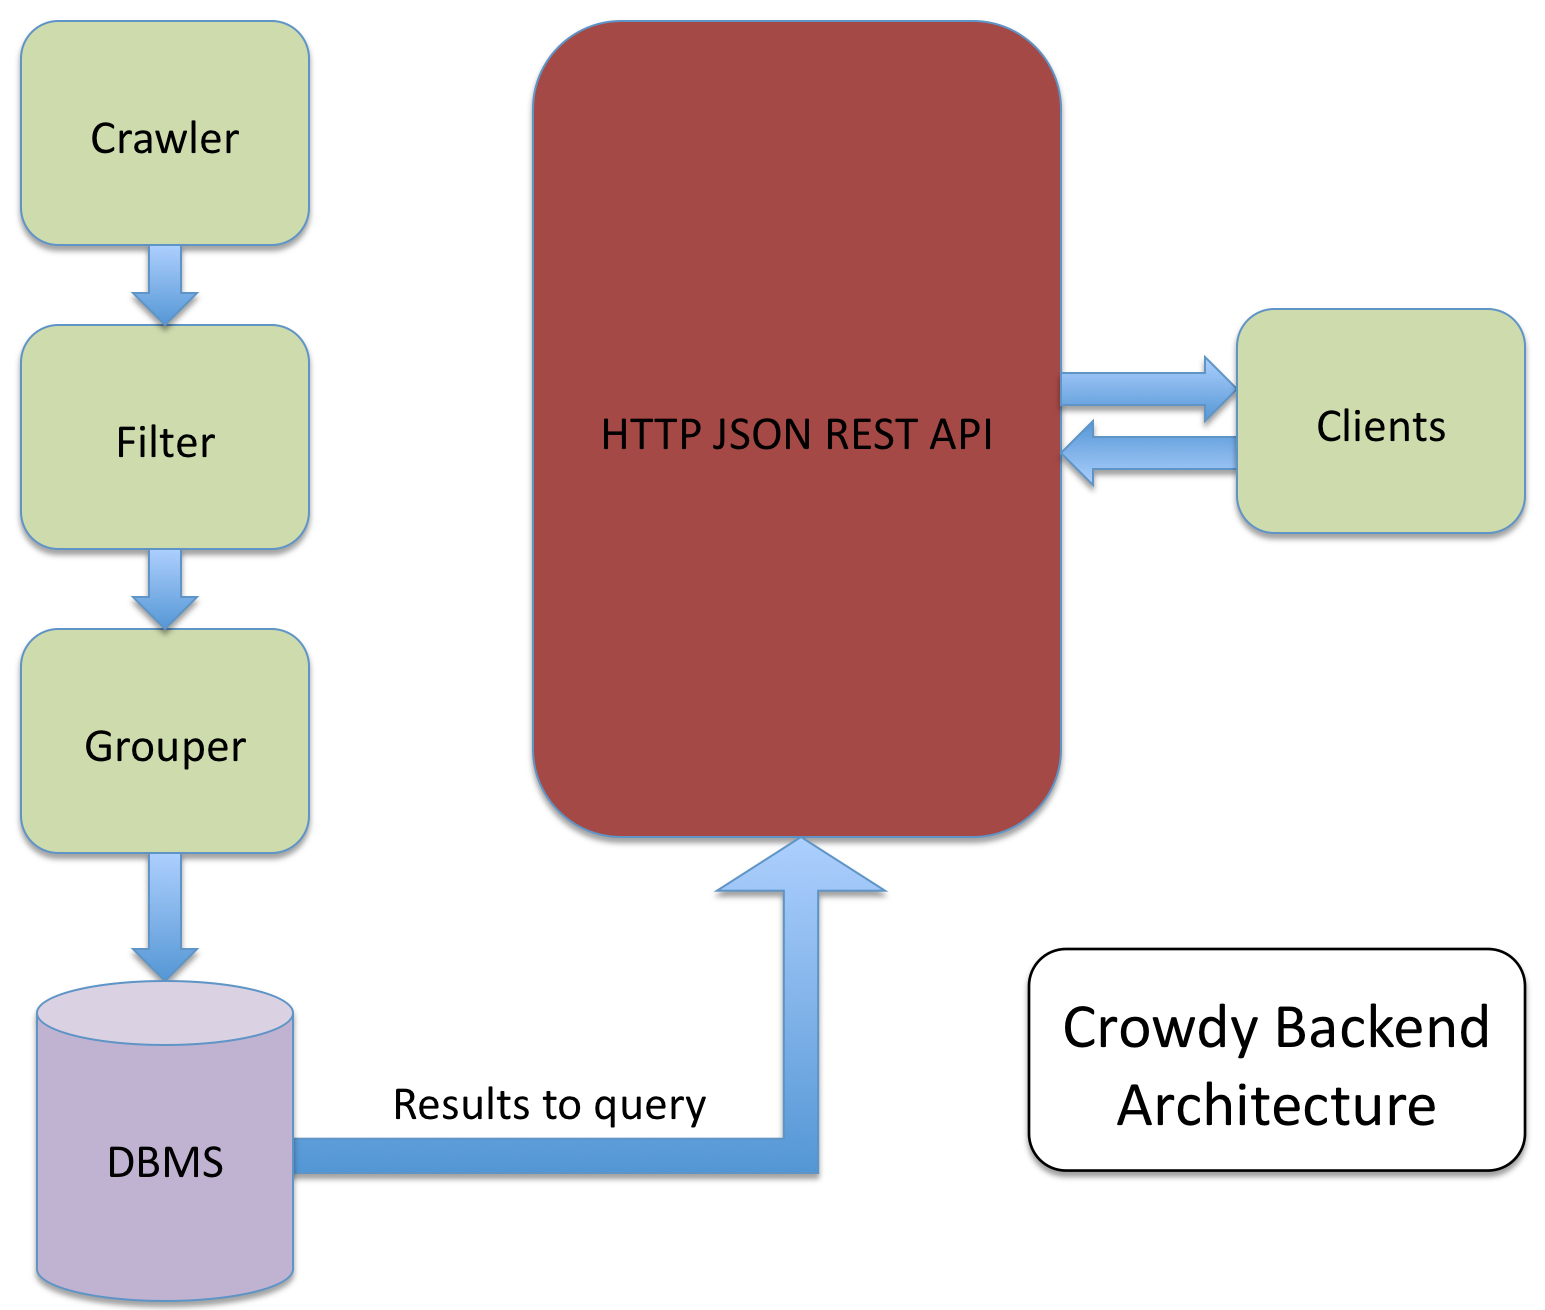
\includegraphics[width=3.0in]{images/architecture}
\caption{Examples for trending phrases discovery problem.}
\label{fig:candidate_phrases}
\end{center}
\end{figure}

An architecture for the proposed solution is shown in Figure 1. The various modules of this architecture are as follows:

\medskip \noindent \textbf{Crawler}: This module deals with interacting with social media websites to collect information. For this project we will be collecting data from Twitter using Twitter Streaming APIs. We collected tweets from [xxxx] users. To collect this set of users we started with a set of 5 users and used snowball sampling to collect more users. We then used used the ``follow'' parameter of the filter method from Streaming API to generate a data stream for crowd detection.

\medskip \noindent \textbf{Grouper}: The grouper module analyses the data collected, to determine crowds and adds them to the DBMS. This is the central module that detects crowds of different types - communication, content, geo-graphical, etc. In this project we will be discovering crowds based on communication only. The algorithm to discover crowds is described in Section~\ref{sec:crowd_algorithm}. Once crowds are discovered, this module formats crowds to a well defined crowds object and adds it to a DBMS.

\medskip \noindent \textbf{Filter}: This module is used to filter un-necessary data from the framework. It can appear both before and after the grouper module depending upon its funcationality. In the figure we have showed the module appear before grouper only. When the module appears before the grouper, it is used to weed out information unnecessary for the grouper. For example in case of crowd detection, it remove information like spam messages. When the module appears after the grouper, it cleans the data generated by the grouper. For, example in case of crowd detection, it analyzes crowds discovered by the grouper and removes un-necessary crowds, or crowds that don't meet specific quality guarentees. The module can also have additional functions that support features like search.

\medskip \noindent \textbf{HTTP JSON RESTful APIs}: This module provides client an interface to the digital library. The module exposes JSON APIs that the clients can use to browze and search the crowds archive.

\begin{itemize}
  \item \noindent\textbf{Beanstalk}: Beanstalk is a simple, fast work queue. We use it to connect the crawlers, filters, and groupers together.
   \item \noindent\textbf{Tornado}: Tornado is an open source, non-blocking web server.  We choose it because it is fast and scalable.
   \item \noindent\textbf{MongoDB}: MongoDB is a scalable, high-performance, open source, document-oriented database. We store the crowds discovered by the framework in this DB. The API module interacts with this database to retrieve collections as required by the user query.
\end{itemize}

\section{Conclusion}
\label{sec:conclusion}

{\scriptsize
 \bibliographystyle{abbrv}
 \bibliography{sigproc}
}
\balancecolumns % GM July 2000

\end{document}
